\documentclass[12pt,a4paper,bibliography=totocnumbered,listof=totocnumbered]{article}
\DeclareMathSizes{12}{12}{12}{12}
\usepackage[ngerman]{babel}
\usepackage[utf8]{inputenc}
\usepackage{amsmath}
\usepackage{amsfonts}
\usepackage{amssymb}
\usepackage{graphicx}
\usepackage{fancyhdr}
\usepackage{tabularx}
\usepackage{geometry}
\usepackage{setspace}
\usepackage[right]{eurosym}
\usepackage[printonlyused]{acronym}
\usepackage{subfig}
\usepackage{floatflt}
\usepackage[usenames,dvipsnames]{color}
\usepackage{colortbl}
\usepackage{paralist}
\usepackage{array}
%\usepackage{titlesec}
\usepackage{parskip}
\usepackage[right]{eurosym}
%\usepackage{picins}
\usepackage[subfigure,titles]{tocloft}
\usepackage[pdfpagelabels=true]{hyperref}
\usepackage{float}

\usepackage{listings}
\lstset{basicstyle=\footnotesize, captionpos=b, breaklines=true, showstringspaces=false, tabsize=2, frame=lines, numbers=left, numberstyle=\tiny, xleftmargin=2em, framexleftmargin=2em}
\makeatletter
\def\l@lstlisting#1#2{\@dottedtocline{1}{0em}{1em}{\hspace{1,5em} Lst. #1}{#2}}
\makeatother

\geometry{a4paper, top=27mm, left=20mm, right=20mm, bottom=35mm, headsep=10mm, footskip=12mm}


\hypersetup{unicode=false, pdftoolbar=true, pdfmenubar=true, pdffitwindow=false, pdfstartview={FitH},
	pdftitle={Wahlpflichtfach: Implementierung von Brettspielen am Beispiel ReversiXT (SS \the\year)},
	pdfauthor={Dr.\ Carsten Kern},
	pdfsubject={Projektbericht},
	pdfcreator={\LaTeX\ with package \flqq hyperref\frqq},
	pdfproducer={pdfTeX \the\pdftexversion.\pdftexrevision},
	pdfkeywords={Projektbericht, ReversiXT},
	pdfnewwindow=true,
	colorlinks=true,linkcolor=black,citecolor=black,filecolor=magenta,urlcolor=black}
\pdfinfo{/CreationDate (D:20151500000000)}
%\titlespacing{\section}{0pt}{12pt plus 4pt minus 2pt}{-6pt plus 2pt minus 2pt}

% Kopf- und Fusszeile
\renewcommand{\sectionmark}[1]{\markright{#1}}
\renewcommand{\leftmark}{\rightmark}
\pagestyle{fancy}
\lhead{}
\chead{}
\rhead{\thesection\space\contentsname}
\lfoot{Implementierung von Brettspielen am Beispiel ReversiXT -- SS \the\year}
\cfoot{}
\rfoot{\ \linebreak Seite \thepage}
\renewcommand{\headrulewidth}{0.4pt}
\renewcommand{\footrulewidth}{0.4pt}

% Vorspann
\renewcommand{\thesection}{\Roman{section}}
\renewcommand{\theHsection}{\Roman{section}}
\pagenumbering{Roman}

\newcommand{\folgen}[1]{
\ensuremath
#1
}

\newcommand{\MyTitlepage}[5][\empty]{
\thispagestyle{empty}
\begin{center}
	
\includegraphics[scale=0.2]{pics/oth-logo.png}\\
	\vspace*{2cm}
	\Large
	\textbf{Fakultät}\\
	\textbf{Informatik und Mathematik}\\
	\vspace*{2cm}
	\Huge
	\textbf{Projektbericht}\\
	\vspace*{0.5cm}
	\large
	zum Wahlpflichtfach im SS \the\year\\
	\vspace*{1cm}
	\textbf{Implementierung von Brettspielen am Beispiel ReversiXT}\\
	\vspace*{1cm}
	\includegraphics[height=6cm]{#1}
	\vfill
	\normalsize
	%\newcolumntype{x}[1]{>{\raggedleft\arraybackslash\hspace{0pt}}p{#1}}
	\begin{tabular}{rl}%{6cm}p{7.5cm}}
	    \rule{0mm}{5ex}\textbf{Gruppe:} & #2 \\
		\rule{0mm}{5ex}\textbf{Autoren:} & \hspace*{-0.5em}\begin{tabular}[t]{r}#3\end{tabular} \\ 
		\rule{0mm}{5ex}\textbf{Leiter:} & Prof. Dr. rer. nat. Carsten Kern \\ 
		\rule{0mm}{5ex}\textbf{Abgabedatum:} & #4 \\ 
	\end{tabular} 
\end{center}
\pagebreak
}

\begin{document}

% ----------------------------------------------------------------------------------------------------------
% Titelseite
% ----------------------------------------------------------------------------------------------------------
\MyTitlepage[pics/gruppenbild]{05}{
\texttt{robin.jahn@st.oth-regensburg.de}\\
\texttt{simon1.melcher@st.oth-regensburg.de}\\
\texttt{alexander1.wess@st.oth-regensburg.de}}
{27.06.\the\year}

\setcounter{page}{1} 
% ----------------------------------------------------------------------------------------------------------
% Inhaltsverzeichnis
% ----------------------------------------------------------------------------------------------------------
\tableofcontents
\pagebreak


% ----------------------------------------------------------------------------------------------------------
% Inhalt
% ----------------------------------------------------------------------------------------------------------
% Abstände Überschrift
%\titlespacing{\section}{0pt}{12pt plus 4pt minus 2pt}{6pt plus 2pt minus 2pt}
%\titlespacing{\subsection}{0pt}{12pt plus 4pt minus 2pt}{4pt plus 2pt minus 2pt}
%\titlespacing{\subsubsection}{0pt}{12pt plus 4pt minus 2pt}{2pt plus 2pt minus 2pt}

% Kopfzeile
\renewcommand{\sectionmark}[1]{\markright{#1}}
\renewcommand{\subsectionmark}[1]{}
\renewcommand{\subsubsectionmark}[1]{}
\lhead{Kapitel \thesection}
\rhead{\rightmark}

\onehalfspacing
\renewcommand{\thesection}{\arabic{section}}
\renewcommand{\theHsection}{\arabic{section}}
\setcounter{section}{0}
\pagenumbering{arabic}
\setcounter{page}{1}

% ----------------------------------------------------------------------------------
% Kapitel: Einleitung
% ----------------------------------------------------------------------------------
\section{Einleitung} \label{kap:Einleitung}
Der Begriff der \glqq künstlichen Intelligenz\grqq{} (kurz K.I.) ist heutzutage allgegenwärtig und findet in der Praxis immer mehr Anwendung, wodurch sich die Nachfrage an diesem Themengebiet erhöht.\cite{ki} Das Wahlpflichtfach \glqq ZOCK - Projekt Client-K.I.s für Brettspiele\grqq{} soll Studierenden einen ersten Einblick in die Algorithmen der künstlichen Intelligenz gewähren. Zur Umsetzung der Lernziele soll ein Projekt in Form einer Client-K.I. für das Spiel ReversiXT erstellt werden, wozu die Teilnehmer in Gruppen von je drei Studierenden aufgeteilt werden. 

Das Spiel ReversiXT basiert auf dem Brettspiel Reversi aus den 1880er Jahren\cite{reversi} und wurde um einige Sonderregelungen erweitert, um dessen Komplexität zu steigern, damit umfassendere K.I.'s entwickelt werden können. Das Original wird von zwei Spielern auf einem acht mal acht Spielfeld gespielt, wie es in Abbildung \ref{fig:reversi_original_map} zu sehen ist, während es in der weiterentwickelten Version möglich ist, auf Karten mit bis zu 2500 Felder, also 50 mal 50, mit höchstens acht Spielern zu spielen. Ein Beispiel eines solchen Spielfelds wird in Abbildung \ref{fig:reversixt_circle_map} dargestellt. Hierbei handelt es sich um eine Karte für drei Spieler mit einer Höhe und Breite von je 29 Feldern, wobei auch verdeutlicht wird, dass Spielfelder nicht zwangsläufig quadratisch sein müssen, sondern individuell gestaltet werden können.

\vspace{1em}
\begin{minipage}{\linewidth}
	\centering
	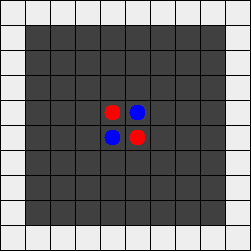
\includegraphics[width=0.4\linewidth]{pics/reversi_original_map.png}
	\captionof{figure}[Reversi Karte]{Originales Spielfeld Reversi}
	\label{fig:reversi_original_map}
\end{minipage}
\\

\vspace{1em}
\begin{minipage}{\linewidth}
	\centering
	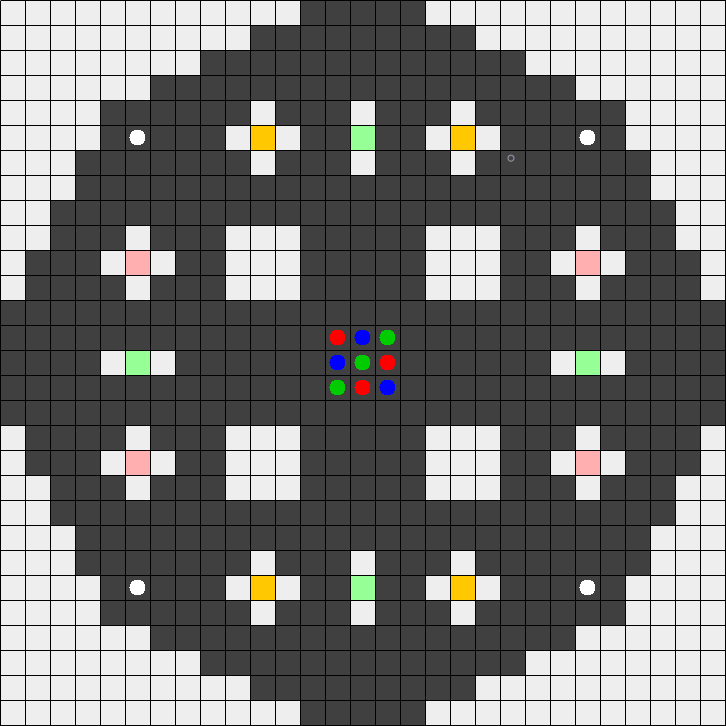
\includegraphics[width=0.7\linewidth]{pics/reversixt_circle_map.png}
	\captionof{figure}[ReversiXT Circle Karte]{Spielfeld ReversiXT}
	\label{fig:reversixt_circle_map}
\end{minipage}
\\

Jedem Spieler werden zu Beginn eine Farbe und somit die dazugehörigen Spielsteine zugewiesen. Das Spielprinzip ist dann, von den eigenen Steinen aus über die Steine der Gegner auf ein freies Feld zu legen, wodurch die eingeschlossenen gegnerischen Steine eingefärbt werden und den Besitzer wechseln. Dies bedeutet, dass zwischen dem eigenen Stein und dem freien Feld immer mindestens ein gegnerischer liegen muss. Es kann generell in jede Richtung, also horizontal, vertikal und diagonal gezogen werden. Ein Beispiel hierfür ist in den folgenden Abbildungen zu sehen wobei Abbildung \ref{fig:capture_pre} die Situation vor dem Zug des Spielers mit den roten Steinen zeigt und durch die weiße Umrandung verdeutlicht werden soll, auf welches Feld gezogen wird. Abbildung \ref{fig:capture_post} stellt den Spielfeldzustand nach dem Färben dar.

\begin{figure}[H]
\centering
\begin{minipage}[c]{0.4\textwidth}
	\centering
	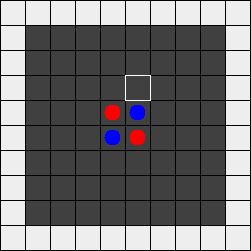
\includegraphics[width=\textwidth]{pics/reversi_original_map_capture_1.png}
	\captionof{figure}[Einfärbern vorher]{Einfärben vor dem Zug}
	\label{fig:capture_pre}
\end{minipage}
\hspace{0.1\textwidth}
\begin{minipage}[c]{0.4\textwidth}
	\centering
	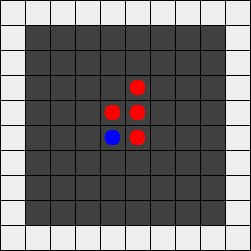
\includegraphics[width=\textwidth]{pics/reversi_original_map_capture_2.png}
	\captionof{figure}[Einfärbern nachher]{Einfärben nach dem Zug}
	\label{fig:capture_post}
\end{minipage}
\end{figure}

Die erweiterte Variante bietet eine zusätzliche Besonderheit bei der Möglichkeit einen gültigen Zug durchzuführen, in Form von sogenannten Überschreibzügen. Diese erlauben es nicht nur auf freie Felder zu legen, sondern auch auf eigene oder gegnerische Steine, um diese einzunehmen, sofern es sich um einen ansonsten regelkonformen Spielzug handelt. Wie viele dieser Steine jeder Spieler zu Beginn zur Verfügung hat, wird vom Ersteller der Karte vorgeschrieben. Es ist jedoch möglich - abhängig vom Spielfeld - zusätzliche Überschreibsteine im Laufe der Runde zu erhalten, worauf im Weiteren noch genauer eingegangen wird. 

Außerdem können ReversiXT Karten besondere Felder enthalten, die ausgelöst werden, sobald ein Spieler das erste Mal darauf zieht. Dazu gehören die Bonusfelder, die dem Spieler die Wahl zwischen einer zusätzlichen Bombe, auf die später noch eingegangen wird, oder eines Überschreibsteins gibt (In Abbildung \ref{fig:reversixt_circle_map} in Gelb dargestellt). Setzt ein Spieler auf ein Inversionsfeld, werden die Farben der Spieler um eins verschoben, wodurch bspw. Spieler 2 die Steine von Spieler 1, Spieler 3 die von Spieler 2 und Spieler 1 die von Spieler 3 erhält (in Abbildung \ref{fig:reversixt_circle_map} in Rosa). Ein Wahlfeld gibt einem Spieler die Möglichkeit seine Steine gezielt mit denen eines Gegners zu tauschen, allerdings kann auch darauf verzichtet werden, indem mit den eigenen Steinen \glqq getauscht\grqq{} wird (In Abbildung \ref{fig:reversixt_circle_map} in Grün). Als letzte Art von Sonderfeldern sind die Expansionsfelder zu nennen, die für alle Spieler als Gegner gelten. Eine weitere Besonderheit dieser Felder ist, dass sie zu jeder Zeit mit einem Überschreibstein eingenommen werden können, selbst wenn dadurch kein gültiger Zug entsteht (In Abbildung \ref{fig:reversixt_circle_map} als weiße Spieler dargestellt). Durch diese Steine können einige interessante Spielfelder entstehen. Es können z. B. Spielfelder gebaut werden, bei denen die Spieler zu Beginn keine eigenen Steine besitzen, es jedoch einige Expansionsfelder gibt. In diesem Fall könnten sich die Spieler in den ersten Zügen aussuchen, auf welchen Expansionsstein sie ziehen möchten. Dieser Ansatz wurde bei der Karte in Abbildung \ref{fig:reversixt_islands_map} verfolgt. Eine weitere Konsequenz von Expansionsfeldern ist, dass abgeschnittene Bereiche einer Karte bespielbar werden, solange dort einige Expansionssteine platziert wurden.

Eine andere Eigenart von ReversiXT sind die Transitionen, die wie eine Art Portal betrachtet werden können. Sie erlauben es über die Wände der Karte hinaus zu ziehen, um an einer andere Stelle der Karte - das andere Ende der Transition - herauszukommen. Diese sind ebenfalls optional und können vom Ersteller des jeweiligen Spielfelds gezielt gesetzt werden. Dadurch können Karten bspw. in einzelne Bereiche eingeteilt werden, die nur über Transitionen erreicht werden können, wie es in Abbildung \ref{fig:reversixt_islands_map} dargestellt wird. Die Transitionen werden hierbei durch gelbe Linien repräsentiert und bestehen aus einem Ein- und Ausgangsfeld sowie einer Richtung in die diese Transition gültig ist. Ebenso ist zu beachten, dass diese sowohl von der einen als auch von der anderen Seite durchlaufen werden kann.

\vspace{1em}
\begin{minipage}{\linewidth}
	\centering
	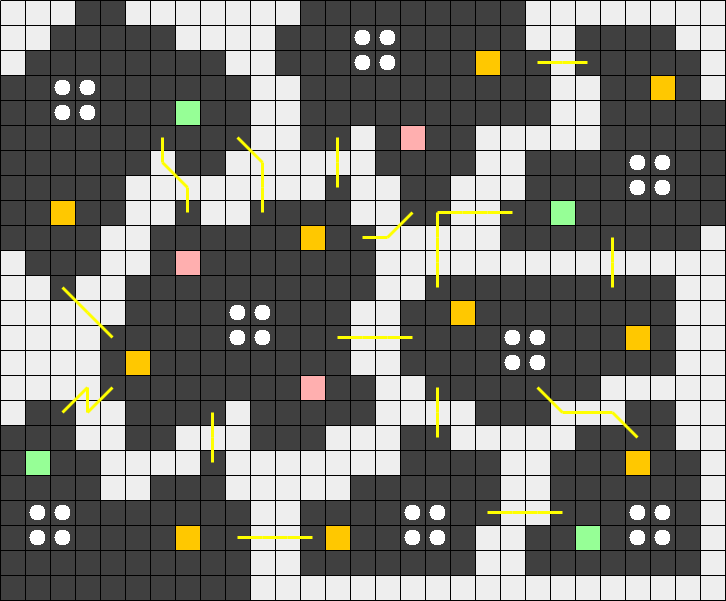
\includegraphics[width=0.7\linewidth]{pics/reversixt_islands_map.png}
	\captionof{figure}[ReversiXT Islands Karte]{Spielfeld mit Transitionen}
	\label{fig:reversixt_islands_map}
\end{minipage}
\\

Aufgrund dieser Besonderheit ist es möglich in Schleifen über die Karte zu gehen, weshalb besonders bei der Durchführung von Zügen darauf geachtet werden muss, dass keine ungültigen Züge getätigt werden. Abbildung \ref{fig:example_transition_loop} zeigt eine solche Situation beispielhaft. Sollte ein Spieler auf das dort dargestellte Expansionsfeld mit einem Überschreibstein ziehen, dürfen die blauen Steine nicht eingefärbt werden, da er sie zwar über die Transition einschließt, dies jedoch mit ein und demselben Stein macht, was gegen die Regeln verstößt.

\vspace{1em}
\begin{minipage}{\linewidth}
	\centering
	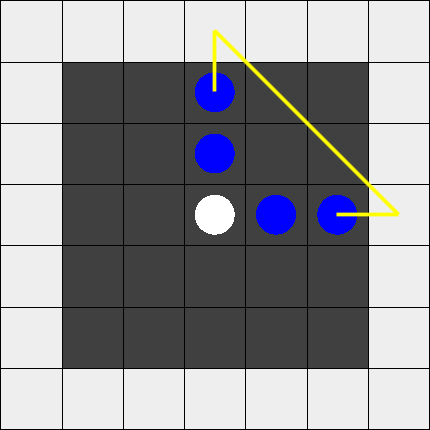
\includegraphics[width=0.4\linewidth]{pics/transition_loop.png}
	\captionof{figure}[Transition loop]{Transition mit Schleife}
	\label{fig:example_transition_loop}
\end{minipage}
\\

Das Spiel endet sobald kein Spieler mehr einen gültigen Zug machen kann. In der herkömmlichen Version gewinnt an dieser Stelle der Spieler, der die meisten Steine einfärben konnte. ReversiXT erweitert das Spielprinzip um eine weiter Spielphase, in der Bomben geworfen werden können. Die Anzahl, wie viele Bomben jeder Spieler initial besitzt sowie deren Stärke, wird zu Beginn der Partie festgelegt und kann je nach Spielfeld variieren. Bomben der Stärke zwei zerstören bspw. das Feld an dem sie platziert werden sowie alle Felder, die innerhalb von zwei Schritten vom Zentrum aus erreichbar sind. Dabei kann auch über Transitionen hinweg gegangen werden, wodurch diese ebenfalls entfernt werden. Deshalb können Bomben eine wertvolle Ressource darstellen, da sie gezielt auf die gegnerischen Steine eingesetzt werden können. Nach dieser Phase wird der Sieger wie im klassischen Reversi bestimmt.


\newpage
% ----------------------------------------------------------------------------------
% Kapitel: Allgemeine Informationen
% ----------------------------------------------------------------------------------
\section{Allgemeine Informationen}
Wie in Kapitel \ref{kap:Einleitung} erwähnt, wurde das Projekt in einer Kleingruppe von drei Studierenden durchgeführt. In diesem Kapitel wird darauf eingegangen, wer Teil der Gruppe 05 war, welche Vorkenntnisse vorhanden waren, wie kommuniziert wurde sowie welche technische Mittel im Hinblick auf die Soft- und Hardware verwendet wurden. Dies soll einen Einblick gewähren, auf welcher Basis das Projekt umgesetzt wurde.

\subsection{Team und Kommunikation}
Die Mitglieder der Gruppe 05 waren Simon Melcher, Robin Jahn und Alexander Wess, die sich alle im vierten Semester ihres Bachelor Informatik Studiums befanden.

Wichtiges Vorwissen wurde vor allem aus den Fächern Programmieren 2 und Algorithmen und Datenstrukturen von den Studierenden mitgebracht. Dort wurde unter anderem anhand von Java die Objektorientierte-Programmierung vermittelt, anhand dieser dann verschiedenste Algorithmen in anderen Modulen besprochen und eigene Projekte durchgeführt wurden. Außerdem wurde ein Grundverständnis über die Komplexität von Algorithmen mitgebracht, wodurch stärker auf Performance geachtet wurde und Einschätzungen getroffen werden konnten, welche Datenstruktur an welcher Stelle sinnvoll war. Robin Jahn konnte sich bereits im Vorfeld wissen zu verschiedenen K.\,I.\ relevanten Themen durch den Austausch mit anderen Studierenden des Studiengangs \glqq Künstliche Intelligenz und Data Science\grqq{} an der OTH Regensburg aneignen.

Neben der wöchentlichen Vorlesung und Übung der Veranstaltung, wurde jeden Freitag eine Besprechung mit allen Mitgliedern abgehalten. In diesen Besprechungen wurden die Aufgaben, die bereits in der Übung am Dienstag verteilt wurden, besprochen und aufgetretene Probleme gemeinsam gelöst. Außerdem wurden neue Ansätze zur Ausarbeitung bzw. Verbesserung des Clients diskutiert und implementiert, sowie neue Aufgaben zur Bearbeitung über das Wochenende zugeteilt. Zusätzlich wurde über eine gemeinsame WhatsApp Gruppe kommuniziert, in der Fragen gestellt werden konnten und organisatorisches vereinbart wurde.

\newpage

\subsection{Wochenübersicht}
\underline{Woche 1:}
\begin{itemize}
\item Robin: Map Datenstruktur implementiert
\item gesamte Gruppe: je zwei Spielfelder erstellt
\end{itemize}
\underline{Woche 2:}
\begin{itemize}
\item Robin: Algorithmus für gültige Züge
\item Simon: Algorithmus für gültige Züge (Spezialfelder)
\item Alex: Beschreibung der Zugheuristik im Projektbericht
\end{itemize}
\underline{Woche 3:}
\begin{itemize}
\item Robin: Umsetzung der verbesserten Heuristik
\item Simon: Git Struktur anhand der Vorgaben angepasst
\item Alex: Projektbericht Kapitel 1 - 3
\end{itemize}
\underline{Woche 4:}
\begin{itemize}
\item Robin: Netzwerkfunktion implementiert, Bombenphase implementiert
\item Simon: Krank
\item Alex: Build-File erstellt
\end{itemize}
\underline{Woche 5:}
\begin{itemize}
\item Robin: Paranoidsuche implementiert
\item Simon: Client Parameter implementiert, Vergleichsmöglichkeit mit der Ausgabe des Servers angelegt
\end{itemize}
\underline{Woche 6:}
\begin{itemize}
\item Robin: Statistiken implementiert
\item Simon: Read Me für Vergleichsskript erstellt und Skript weiterentwickelt
\item Alex: Alpha-Beta-Pruning implementiert
\end{itemize}
\underline{Woche 7:}
\begin{itemize}
\item Robin: Zugsortierung implementiert, Skript zur Ermittlung der besten Multiplikatoren erstellt
\item Simon: Iterative-Deepening implementiert
\item Alex: Erweiterung des Projektberichts
\end{itemize}
\underline{Woche 8:}
\begin{itemize}
\item Robin: Überarbeitung Skripte
\item Simon: Funktion für die Bombenphase zum Zählen der Steine entwickelt
\item Alex: Funktion zur Bewertung von Bonusfeldern erstellt
\item gesamte Gruppe: ToDo's abgearbeitet
\end{itemize}
\underline{Woche 9:}
\begin{itemize}
\item Robin: Aufteilung Map Klasse in statischen und dynamischen Teil, neue Suchbaum Klasse
\item Simon: BRS+, Killer Heuristik und Phasen für Heuristik implementiert
\item Alex: BRS+ implementiert
\end{itemize}
\underline{Woche 10:}
\begin{itemize}
\item Robin: Entwurf Algorithmus erreichbare Felder, MCTS implementiert
\item Simon: Implementierung Algorithmus erreichbare Felder, Zobrist Hashing und Aspiration Window implementiert
\item Alex: Methode zufälliger Zug implementiert
\end{itemize}
\underline{Wochen 11 - 13:}
\begin{itemize}
\item Robin: Disqualifikation beseitigt (ein Überschreibzug zu viel), Aufteilung Heuristik in statisch und dynamisch, Wellen dynamisch gemacht, Vader Map erstellt
\item Simon: Alderan Map erstellt, testen der optionalen Optimierungen (Zobrist Hashing und Aspiration Window)
\item Alex: Zufälliger Zug überarbeitet (Suche in Spirale), Projektbericht überarbeitet
\item gesamte Gruppe: Optimierungen und Erweiterung Projektbericht
\end{itemize}

\newpage

\subsection{Technische Daten}
In diesem Abschnitt soll auf die verwendeten technischen Mittel eingegangen werden. Das Projekt wurde in der Programmiersprache Java auf dem Stand der 11ten Version umgesetzt. Zum einen wurden in dieser Programmiersprache bereits die meisten Erfahrungen gesammelt. Zum anderen konnten auch die gängigen Vorteile von Java genutzt werden, wie z. B. die automatische Speicher- und Heap-Verwaltung oder die Möglichkeit mit \glqq Call by Reference\grqq{} zu arbeiten ohne Pointer zu benutzen.
Zu Beginn legte sich die Gruppe fest, einheitlich die Entwicklungsumgebung IntelliJ IDEA der Version 2021.3.3 von JetBrains zu nutzen. Der Vorteil davon war unter anderem, dass diese bereits eine gute Anbindung an Git besaß und somit das Arbeiten in einem gemeinsam Repository signifikant erleichterte.
Als Betriebssystem wurde hauptsächlich Windows 10 der Version 21H2 verwendet. Außerdem wurde von Robin Jahn eine virtuelle Maschine (VM) eingerichtet, die das Unix Betriebssystem Ubuntu simulierte. Simon Melcher und Alexander Wess nutzten hingegen das Windows Subsystem for Linux (WSL). Einerseits konnte mittels Linux der Server ausgeführt werden, wodurch neuer Code direkt im Spiel ausprobiert werden konnte. Andererseits konnten durch die Verwendung von WLS und der VM unterschiedliche Probleme identifiziert werden, die spezifisch auf einer der Umgebungen aufgetreten sind. Dadurch sollte sichergestellt werden, dass der entwickelte Client fehlerlos über ein Linux Betriebssystem ausgeführt werden konnte und die Kommunikation mit dem Server reibungslos funktionierte.

Ebenfalls wurden die Tools aus dem globalen Repository wie der Map Editor genutzt, um Spielfelder zu erstellen und zu bearbeiten. Zusätzlich wurden Skripte angefertigt, die die Erstellung des Projekts erleichtern sollten. Um den Server, auf dem die Spiele ausgetragen wurden und die zur Verfügung gestellte triviale K.I., nicht nach jedem Spiel neu starten zu müssen, wurde ein Skript geschrieben, welches dies übernahm. Zur Verbesserung der Heuristik, die in Kapitel \ref{kap:Heuristik_Beschreibung} genauer beschrieben wird, wurde ein weiteres Skript entwickelt. Dieses wurde verwendet, um möglichst gute Multiplikatoren der einzelnen Heuristik Bestandteile herauszufinden. Die Umsetzung erfolgte, indem zu Beginn einer Partie alle Multiplikatoren zufällig in einem definierten Bereich gesetzt wurden. Dann wurden drei Spiele gespielt, um diese zu testen, eines auf einer zwei Spieler Karte, eines mit vier Spielern und eins mit acht. Hierbei spielte der eigene Client immer gegen triviale KI's. Nach den drei Spielen wurde die mittlere Platzierung bestimmt und geprüft, ob ein neuer Höchstwert erzielt wurde. Um die Effizienz des Skripts zu Steigern, wurden einerseits nur die eben erwähnten drei Karten bespielt und andererseits wurden Partien abgebrochen, wenn der eigene Client letzter wurde.

Robin Jahn entwickelte zu Beginn auf seinem Laptop mit einem AMD Ryzen 5 3500U Prozessor, der eine Taktfrequenz von 2,1 bis 3,7 GHz aufwies und 8 GB Arbeitsspeicher besaß. Jedoch wechselte er, vor allem zum Testen, auf seinen Tower PC, der mit einem Intel Core i5-7600 (3,5 GHz), 16GB RAM und einer Nvidia GeForce GTX 1070 Grafikkarte ausgestattet war, da dieser die virtuelle Maschine aufgrund seiner höheren Leistung besser bewältigen konnte. Simon Melcher wechselte ebenfalls zwischen einem Desktop Computer und einem Laptop für die Vorlesungen, Übungen und Gruppenmeetings. Beide Geräte besaßen 16 GB RAM sowie einen AMD Ryzen 5 2600X (3,6 GHz), der in seinem PC enthalten war und einen AMD Ryzen 3500U (2,1 GHz) in seinem Laptop. Alexander Wess arbeitet durchgehend mit einem Laptop, der einen AMD Ryzen 5 5500U (2.10 GHz) Prozessor und 16 GB Arbeitsspeicher verbaut hatte.

\newpage
% ----------------------------------------------------------------------------------
% Kapitel: Spielfeldbewertung
% ----------------------------------------------------------------------------------
\section{Spielfeldbewertung} \label{kap:Spielfeldbewertung}
Zur Umsetzung eines solchen Clients wird eine K.I. benötigt, die anhand von Suchbäumen entscheidet, welcher Zug als nächstes getätigt werden soll. Die Elemente dieses Suchbaums sind verschiedene Szenarien, die aus der aktuellen Situation auf dem Spielfeld entstehen können. Hierfür müssen die verschiedenen Zugmöglichkeiten simuliert und der daraus entstandene Zustand bewertet werden, um zu entscheiden, welcher der bestmögliche Zug ist.
In diesem Kapitel soll deshalb darauf eingegangen werden, wie Gruppe 05 diese Einschätzung umgesetzt hat.

\subsection{Bestandteile}\label{kap:Heuristik_Beschreibung}
Die wohl einfachste Bewertung eines Spielfelds wäre das Zählen der eigenen Steine in Relation zu denen der Gegner, was in diesem Kontext als Greedy-Verfahren bezeichnet wird. Bei einem solchen Vorgehen achtet der Spieler nur darauf möglichst viele Steine auf dem Feld zu haben bzw. beim Tätigen eines Spielzugs möglichst viele Steine einzufärben.

Eine weitere mögliche Heuristik zur Spielfeldbewertung ist die eigene Flexibilität in Bezug auf durchführbare Spielzüge, die hier auch als "Mobilität" bezeichnet wird. Hierbei ist der Grundgedanke zu berücksichtigen, wie viele Optionen der Spieler hat das Spiel weiterzuführen. Mehr valide Züge als der Gegner zu haben ist dementsprechend von Vorteil. Dadurch soll sichergestellt werden, dass die eigene Strategie weiterverfolgt werden kann und nicht der Gegner den Spielverlauf vorgibt.


Die zuvor beschriebene Situation ist in Abbildung \ref{fig:example_heuristics_flexibility_simple} zu sehen. Der Spieler mit den blauen Steinen hat zwar mehr eingefärbt, kann jedoch nicht mehr ziehen (sofern keine Überschreibsteine verfügbar sind) und muss abwarten, was der Spieler mit den roten Steinen als nächstes macht. Dieser kann hingegen frei entscheiden in welche Richtung die Karte als nächstes bespielt werden soll, da er in mehrere Richtung ziehen kann.

Jedoch bringt dieses Verfahren auch Nachteile mit sich, da das Ziel des Spiels, am Ende der Partie die meisten Steine auf dem Spielfeld zu haben, vernachlässigt wird. Deshalb sollte es mit anderen Bewertungsmethoden kombiniert werden.

\vspace{1em}
\begin{minipage}{\linewidth}
	\centering
	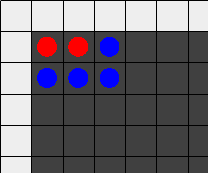
\includegraphics[width=0.3\linewidth]{pics/heuristics_flexibility_simple_v2.png}
	\captionof{figure}[Heuristik Flexibilität]{Situation Blau kann nicht mehr ziehen}
	\label{fig:example_heuristics_flexibility_simple}
\end{minipage}
\\


Zur Umsetzung der Spielfeldbewertung hinsichtlich des Greedy-Verfahrens und der Mobilität wurde das gleiche Vorgehen verwendet. Im Folgenden wird die Umsetzung des Greedy-Verfahrens beschrieben.
Zuerst wird die Anzahl der eigenen Steine und die Anzahl der gefärbten Steine bestimmt. Durch den Quotienten dieser beiden Werte bekommt man den Anteil der eigenen Steine zu allen Steinen, die bisher eingenommen wurden. Wenn man beispielsweise 25 von insgesamt 100 gefärbten Steinen besitzt, hat man 25\% der Steine. Dieser Anteilswert hat jedoch je nach Anzahl der Spieler auf einer Karte eine andere Aussagekraft. Besitzt man 25\% der Steine auf einer 2-Spieler Karte, ist dieser Wert schlecht. Bei einer 4-Spieler Karte ist es jedoch der Durchschnitt. Um dieses Problem zu lösen, wird der Wert normiert, indem er durch die Durchschnittsanzahl der Steine pro Spieler geteilt wird. 

Insgesamt ergibt sich dadurch:
\[ \frac{ \frac{\text{ \# meine Steine}}{\text{ \# gefärbte Steine}} }{ \frac{1}{ \# Spieler} } \]
Was vereinfacht werden kann zu:
\[ \frac{ \text{ \# meine Steine } \cdot \text{ \# Spieler} }{ \text{ \# gefärbte Steine} } \] 
Wenn das Endergebnis 1 ist, bedeutet dies, dass der Spieler genau so viele Steine besitzt, wie er im Durchschnitt besitzen sollte. Ist es 0,5 oder auch 50\% hat der Spieler nur 50\% der Steine, die er im Durchschnitt besitzen sollte. Ebenso hat er bei einem Wert von 1,5 150\% der durchschnittlichen Steine.
Im Vergleich zu einem Absolutwert hat diese Methode einige Vorteile. Da die Werte unabhängig von der Anzahl der Spieler oder des Spielfortschritts sind, kann ein Multiplikator auf den Wert gerechnet werden, um das Gewicht dieser Bewertungsmethode gegenüber den anderen zu verändern. Dieses ist durch die Unabhängigkeit auf allen möglichen Karten gleich, was dem gewünschten Verhalten entspricht.

Wie bereits zuvor erwähnt kann das gleiche Verfahren auch für die Bewertung der Mobilität verwendet werden. In diesem Fall sieht die Formel wie folgt aus:
\[ \frac{ \text{ \# meine Züge } \cdot \text{ \# Spieler } }{ \sum_{i=1}^{ \#Spieler} \text{ \# Züge von Spieler i } }  \]


Ein weiterer Ansatz der Spielfeldbewertung ist die \glqq Sicherheit\grqq{} der einnehmbaren Felder. In diesem Fall soll darauf geachtete werden, ob und wie leicht die jeweiligen Felder vom Gegner eingefärbt werden können. Folglich muss hierbei überprüft werden, ob ein Feld, nachdem es das erste Mal besetzt wird, überhaupt noch einmal den Besitzer wechseln kann oder aus wie vielen Richtungen die Gegner noch Möglichkeiten haben, dieses Feld zurückzugewinnen. Zusätzlich soll einkalkuliert werden, wie viel Prozent der bespielbaren Felder ausgehend von dieser Position erreichbar sind. Diese Analyse wird anhand eines Punktesystems realisiert, auf das im weiteren Verlauf dieses Kapitels noch genauer eingegangen wird.

Das naheliegendste Beispiel für ein solches sicheres Feld ist eine Ecke wie in Abbildung \ref{fig:example_heuristics_safe_fields_corner} dargestellt. Dieser Stein kann weder horizontal noch vertikal oder diagonal von einem Gegner eingefärbt werden und stellt somit eine wertvolle Position dar. Aufgrund der zusätzlichen Regeln von ReversiXT können diese Felder zwar noch mit Überschreibsteine eingenommen werden, jedoch muss dafür eine begrenzte und wertvolle Ressource verwendet werden.

\vspace{1em}
\begin{minipage}{\linewidth}
	\centering
	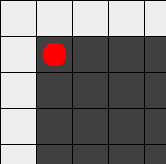
\includegraphics[width=0.3\linewidth]{pics/heuristics_safe_fields_corner.png}
	\captionof{figure}[Heuristik sichere Felder Bsp. 1]{Nicht einnehmbares Feld mit vielen Zugmöglichkeiten}
	\label{fig:example_heuristics_safe_fields_corner}
\end{minipage}
\\

Abbildung \ref{fig:example_heuristics_safe_fields_dead_end} zeigt eine andere Situation, in der das Feld zwar ebenfalls nicht mehr mit einem herkömmlichen Zug eingenommen werden kann, jedoch auch nur eine Richtung (nach Unten) als Zugmöglichkeit bietet. Somit kann von hieraus nur ein geringer Prozentsatz der Karte bespielt werden und sollte schlechter eingestuft werden als das Feld aus der Situation davor.

\vspace{1em}
\begin{minipage}{\linewidth}
	\centering
	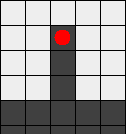
\includegraphics[width=0.3\linewidth]{pics/heuristics_safe_fields_dead_end.png}
	\captionof{figure}[Heuristik sichere Felder Bsp. 2]{Nicht einnehmbares Feld mit wenigen Zugmöglichkeiten}
	\label{fig:example_heuristics_safe_fields_dead_end}
\end{minipage}
\\

Ein Feld, das sich am Rand der Karte befindet, kann zwar eingenommen werden, jedoch sind die Möglichkeiten beschränkt, da es lediglich vertikal von gegnerischen Spielern eingefärbt werden kann, wie es in Abbildung \ref{fig:example_heuristics_safe_fields_outer_side} zu sehen ist. Gleichzeitig eröffnet es Möglichkeiten in fünf Richtungen den nächsten Spielzug durchzuführen.

\vspace{1em}
\begin{minipage}{\linewidth}
	\centering
	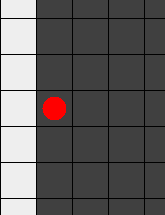
\includegraphics[width=0.3\linewidth]{pics/heuristics_safe_fields_outer_side.png}
	\captionof{figure}[Heuristik sichere Felder Bsp. 3]{Beschränkt einnehmbares Feld}
	\label{fig:example_heuristics_safe_fields_outer_side}
\end{minipage}
\\

Wenn keine Seite durch das Ende der Karte geschützt ist, ist dieses Feld von allen Seiten für den Gegner erreichbar, bietet jedoch gleichzeitig viele Zugmöglichkeiten. Deshalb muss durchdacht werden, wann welche Position wichtiger ist. In Abbildung \ref{fig:example_heuristics_safe_fields_middle} wird dies durch ein Feld inmitten der Spielfläche verdeutlicht.

\vspace{1em}
\begin{minipage}{\linewidth}
	\centering
	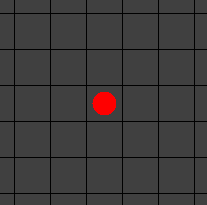
\includegraphics[width=0.3\linewidth]{pics/heuristics_safe_fields_middle.png}
	\captionof{figure}[Heuristik sichere Felder Bsp. 4]{Voll einnehmbares Feld}
	\label{fig:example_heuristics_safe_fields_middle}
\end{minipage}
\\

Die Schwierigkeit dieser Heuristik besteht darin, dass die Sonderregeln von ReversiXT nicht vernachlässigt werden dürfen. Ein vermeintlich sicheres Feld (z. B. eine Ecke), kann durch Transitionen gar kein uneinnehmbares Feld sein und muss auch als dieses behandelt werden. Diesen Effekt können auch Überschreibsteine hervorrufen.

Wie bereits zuvor erwähnt, wurde die Analyse zur Sicherheit der Felder bzw. deren Wert anhand eines Punktesystems realisiert. Hierbei wurde jedem Feld eine Zahl zugeordnet, die auf Basis von einigen Kriterien errechnet wurde und somit darstellt, wie bedeutend dieses ist. Zuvor wurde bereits erläutert, dass zum einen die Möglichkeiten der Gegner zur Eroberung des Feldes, als auch die daraus ausgehenden Wege maßgebend sind. Zusätzlich wurde berücksichtigt, wie weit von den jeweiligen Positionen aus gezogen werden kann, bzw. wie viel Prozent des Spielfelds davon ausgehend erreichbar sind. Dadurch sollte sichergestellt werden, dass Felder, die zwar nicht mehr eingenommen werden können, aber sich bspw. in schmäleren Bereichen der Karte befinden und somit weniger Zugmöglichkeiten bieten, nicht so gut bewertet werden, wie welche von denen aus weit ins Spielfeld hinein gezogen werden kann. Der Stein, der in Abbildung \ref{fig:example_heuristics_reachable_fields} zu sehen ist, ist ein Beispiel für ein solches Feld. Ein gegnerischer Spieler kann diesen Stein zwar nicht mehr erobern, aber gezogen werden kann von hier aus nur nach oben, da links und diagonal nur ein Feld bis zum Ende der Karte ist.

\vspace{1em}
\begin{minipage}{\linewidth}
	\centering
	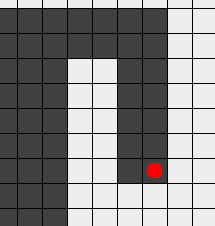
\includegraphics[width=0.5\linewidth]{pics/heuristics_reachable_fields.png}
	\captionof{figure}[Heuristik erreichbare Felder]{Feld mit beschränkten Zugmöglichkeiten}
	\label{fig:example_heuristics_reachable_fields}
\end{minipage}
\\

Ebenso wurden die speziellen Felder von ReversiXT höher eingestuft als normale, sodass bspw. ein Bonusfeld immer eingenommen wird, sofern es möglich ist. Um sicher zu gehen, dass der eigene Client vorteilhafte Felder auch einnehmen kann, wurde ein Algorithmus entworfen, der die angrenzenden Bereiche mit negativen Zahlen gewichtet. Dadurch sollte signalisiert werden, dass diese Felder gemieden werden sollten, da sie dem Spieler die Chance verwehren, auf eines der positiven Felder zu ziehen und nur dem Gegner die Gelegenheit dafür geben würde. Hierbei wurde jedoch darauf geachtet, dass vorteilhafte Felder sich nicht gegenseitig beeinflussen, da z. B. mehrere Bonusfelder, die direkt nebeneinander liegen ansonsten die Bewertung verfälschen würden und möglicherweise sogar geringer eingestuft werden würden als gewöhnliche. Gebiete, die wiederum an solche negativ eingeschätzten Felder angrenzen, wurden wieder positiv beziffert, womit das Ziel verfolgt wurde, dass der eigene Client auf diese zieht, um den Gegner dazu zu bringen, auf ein Feld zu legen, das sich um ein nutzbringendes Feld befindet. Dieses Verfahren von abwechselnden negativen und positiven Bewertungen, ausgehend von dem bedeutenden Feld, wurde weitergeführt, wodurch eine Art Welle entstand.
Im Laufe der Entwicklung zeigte sich, dass eine statische Berechnung dieser Wellen nicht immer gewinnbringend war, da Felder, wie bspw. Bonusfelder weiterhin positiv dargestellt wurden, selbst wenn diese bereits von einem Gegner eingenommen wurden und somit keinen zusätzliche Ressource mehr brachten. Dadurch bevorzugte der Client weiterhin diese Spielfelder z. B. beim Durchführen von Überschreibzügen, obwohl es sich lediglich um ein normales Feld handelte. Deshalb wurde bei Bonusfeldern die Wellen rundherum und der zusätzliche Wert entfernt, sobald es das erste Mal eingenommen wurde.

Abschließend wurden die Werte der einzelnen Heuristikbestandteile addiert. Das Endergebnis einer solchen Berechnung ist in Abbildung \ref{fig:example_heuristics_implementation_field_values_matrix} zu sehen. Hier ist deutlich zu erkennen, dass Felder in den Ecken höher beziffert sind als andere. Außerdem kann festgestellt werden, dass die Bereiche um die Ecken einen deutlich niedrigeren Wert besitzen, was auf die negative Bewertung durch die Wellen zurückzuführen ist.

\vspace{1em}
\begin{minipage}{\linewidth}
	\centering
	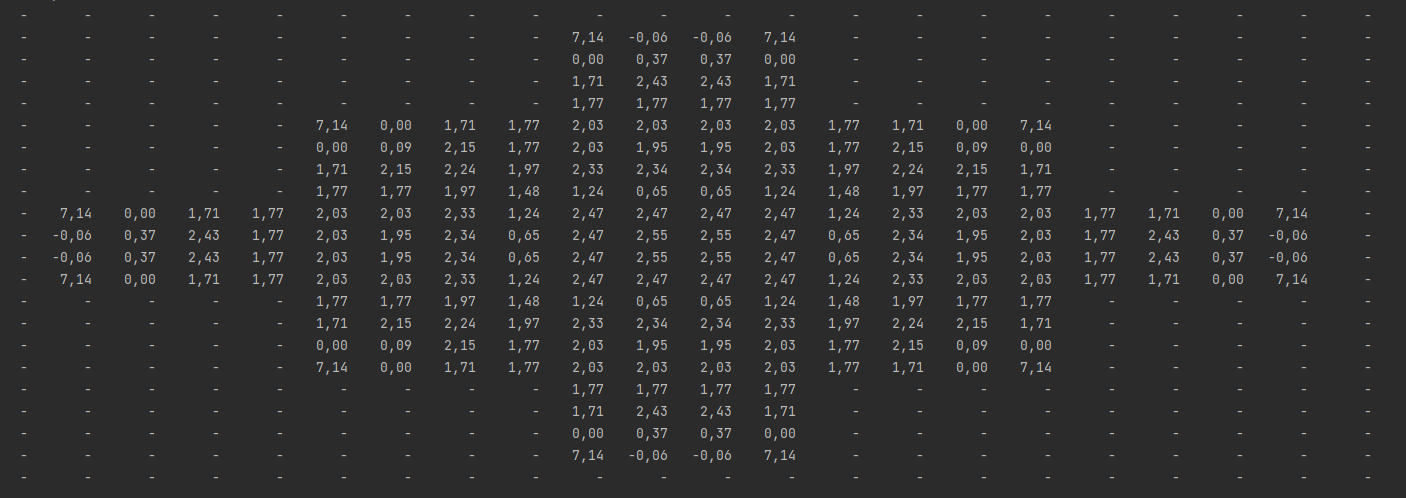
\includegraphics[width=\linewidth]{pics/heuristics_implementation_field_values_matrix.png}
	\captionof{figure}[Heuristik Implementierung Bewertung Felder]{Spielfeld mit Punktzahl zur Bewertung der Felder}
	\label{fig:example_heuristics_implementation_field_values_matrix}
\end{minipage} 
\\

Die einzelnen Komponenten der Heuristik wurden mithilfe von Multiplikatoren verschieden stark priorisiert. Während der Entwicklung des Clients wurde ersichtlich, dass die unterschiedlichen Bewertungsmethoden im Laufe eines Spiels unterschiedlich schwer gewichtet werden sollten. Deshalb wurde ein Algorithmus entworfen, der angibt wie viele Felder auf einer Karte tatsächlich bespielbar sind. Daraufhin wurden verschiedene Phasen implementiert, die angaben, wie weit das Spiel bereits vorangeschritten ist und die Multiplikatoren der einzelnen Heuristiken abhängig davon neu setzte. In der ersten Phase befand sich die Partie solange weniger als 50\% der bespielbaren Felder eingenommen wurden. Verschiedene Tests zum Finden der optimalen Multiplikatoren ergaben, dass zu diesem Zeitpunkt vor allem wichtig war, wie weit von diesem Feld gezogen werden kann. War der Wert der eingefärbten Felder zwischen 50\% und 80\%, befand sich das Spiel in der Mitte und somit in Phase 2. Hier wurde noch zusätzlich der Multiplikator für die Anzahl der einzufärbenden Steine deutlich erhöht, während die anderen kaum verändert wurden. Ab 80\% Füllmenge des Spielbretts wurden die Multiplikatoren für Phase 3 gesetzt, in der die Mobilität an Wichtigkeit zunahm.
 
\newpage
% ----------------------------------------------------------------------------------
% Kapitel: Zusätzliche Inhalte
% ----------------------------------------------------------------------------------
\section{Optimierungen}
Wie schon in Kapitel \ref{kap:Spielfeldbewertung} erwähnt, wird für die Berechnung, welcher der möglichen Züge der Beste ist, ein Suchbaum verwendet. Daher spielt die Tiefe, in die bei der Berechnung vorgedrungen werden kann eine sehr große Rolle. Diese gibt an, wie weit die K.I. in die \glqq Zukunft\grqq{} schauen konnte, um die verschiedenen Züge zu bewerten. Je höher also die Tiefe, desto besser kann bewertet werden, welcher Zug gemacht werden sollte. Verfahren, um diese zu erhöhen sind also ein sehr wichtiger Bestandteil von Suchbaum K.I.'s. Optimierungsverfahren wie Alpha-Beata-Prouning, Move Sorting und BRS+ wurden im Rahmen der Vorlesung implementiert. Um nun den eigenen Client noch weiter zu verbessern, wurden weitere Verfahren implementiert, die im Folgenden beschrieben werden.

\subsection{Look at returned move first}
Wenn ein Spiel auf Zeit gespielt wird, bekommt jeder Spieler für seinen Zug einige Sekunden Rechenzeit. Um sicher zu gehen, dass ein möglichst guter Zug gefunden werden kann, wird das Iterative-Deepening Verfahren verwendet. Beim Vorgehen nach diesem Verfahren wird zuerst ein Zug für Tiefe eins berechnet. Wenn danach noch Zeit übrig ist, wird ein Zug für die nächste Tiefe berechnet und so weiter. Eine Beobachtung, die bei diesem Vorgehen gemacht werden kann ist, dass der beste Zug für die eine Tiefe oft auch der beste Zug für die nächste Tiefe sein wird. Wir können also annehmen, dass der Zug, der für die letzte Tiefe berechnet wurde, auch in der folgenden Tiefe hoch bewertet wird. Wenn dieser Zug nun für die nächste Tiefe jeweils zu Beginn abgehandelt wird, wird am Anfang im Suchbaum ein hoher Wert zurückgegeben. Dies führt dazu, dass das Alpha-Beta-Pruning Verfahren mehr Teilbäume abschneiden kann. Somit benötigt die Berechnung weniger Zeit, die in weitere Berechnungen investiert werden kann.

\subsection{Reachable Fields}
Wie schon an anderer Stelle erwähnt kann es Spielfelder geben, bei denen manche Felder nicht erreicht werden können. Damit diese nicht andere Berechnungen verfälschen, lassen wir am Anfang einen Algorithmus über das Spielfeld laufen, der alle erreichbaren Felder findet. Diejenigen Felder, die nicht erreicht werden können werden im folgenden Spiel als Wand interpretiert, solange es sich in Phase eins befindet. In der Bombenphase müssen die Felder jedoch als normales Feld interpretiert werden, da es auch möglich ist eine Bombe auf ein unerreichbares Feld zu werfen.

\subsection{Aspiration Window}
Die Idee des Aspiration-Window Verfahrens ist es, dass bei Alpha Beta Pruning auf oberster Ebene konkrete Werte für Alpha und Beta eingesetzt werden sollen und nicht -$\infty$ und +$\infty$
Dafür wird der Wert der vorangegangenen Iteration genommen und die Fenstergröße addiert bzw. subtrahiert, wodurch man \textalpha, bzw. \textbeta\ erhält.
Sollte dann ein berechneter Wert nicht in dem Intervall liegen, muss die Suche auf der gleichen Tiefe noch einmal gestartet werden. Diesmal mit komplett geöffneten \textalpha\ und \textbeta\ also -$\infty$ und +$\infty$. Wenn dies eintritt führt es jedoch zu mehr Aufwand als eine Suche, die von Anfang an mit -$\infty$ und +$\infty$ gestartet wurde.

Da ReversiXT ein sehr volatiles Spiel ist, muss eine sehr große Fenstergröße angesetzt werden, um die Anzahl der kompletten Neusuchungen in einen akzeptablen Bereich zu bringen. Dies führt allerdings dazu, dass insgesamt so gut wie kein Zeitgewinn gemacht werden kann.
Deswegen haben wir uns entschieden es generell zu deaktivieren.

\subsection{Transposition Tabelle mit Hilfe von Zobrist Hashing}
Bei der Evaluierung von Karten kann die Rechenzeit verringert werden, indem bereits berechnete Ergebnisse gespeichert werden. Wenn eine Karte nun evaluiert werden soll, kann geprüft werden, ob bereits ein gespeichertes Ergebnis vorliegt. Dies ist über eine Hash-Tabelle realisierbar, wofür aus einer Karte ein Hashwert gebildet werden muss.

Um aus einem Spielbrett einen möglichst einzigartigen Hash in akzeptabler Zeit zu generieren, verwenden wir Zobrist Hashing.

Dafür wird am Anfang eine Zobrist Tabelle erstellt, welche drei Dimensionen besitzt. Die ersten beiden Dimensionen müssen so gewählt werden, dass die Karte darauf abbildbar ist. Die dritte Dimension wird nun dafür verwendet, verschiedene Attribute der Karte abzubilden. In unserem Fall hat die dritte Dimension zwei Elemente, wobei das erste für die eigenen Steine verwendet wird und das zweite für die der Gegner. Zusätzlich dazu wird noch ein Wert gespeichert, der dafür steht, ob der eigene Spieler am Zug ist.

Alle Felder der Zobrist Tabelle werden nun mit zufälligen 64-Bit Zahlen initialisiert.
Um nun den Hashwert für eine gegebene Karte zu ermitteln, wird bei einem Hash Wert von null gestartet. Dann wird in Reihenfolge über jedes Feld der Karte gelaufen und der entsprechende Wert aus der Zobrist Tabelle geholt. Wenn es beispielsweise ein gegnerisches Feld ist, gehört dieses zum zweiten Attribut. Demzufolge wird die Tabelle des zweiten Attributs verwendet und der Wert an den entsprechenden Koordinaten verwendet. Dieser Wert wird nun bitweise mittels des XOR Operators auf den aktuellen Wert gerechnet. Nachdem über alle Felder der Karte iteriert wurde, wird in der selben Weise noch der Wert darauf gerechnet, ob der eigene Spieler am Zug sind.

Da die Zobrist Tabelle nur einmal aufgebaut werden muss, kann überlegt werden, ob nicht eine explizit aufgebaute Tabelle verwendet werden sollte, anstatt einmal am Anfang eine zufällige zu generieren.
Da dies jedoch zu anderen Problemen führen würde und der Aufbau einer maximal großen Tabelle gemittelt über 1.000.000 Versuche durchschnittlich nur 3,7 ms braucht, haben wir uns dagegen entschieden.

In der nachfolgenden Tabelle sind die durchschnittlich erreichten Tiefen aufgeführt. Die erste Spalte steht für die Kartengröße und die erste Zeile für die Größe der Transpositionen Tabelle. Null steht hierbei dafür, dass ohne Tabelle gerechnet wurde.

\begin{table}[!h]
\centering
	\begin{tabular} {| m{1.7cm} | m{3cm} | m{3cm} | m{3cm} | m{3cm}|}
		\hline
		\textbf{} &\textbf{0} &\textbf{32000} & \textbf{64000} & \textbf{128000}\\
		\hline
		20x20 & 4,6 & 5,07 & 5,175 & 5,2 \\
		\hline
		50x50 & 2,3 & 2,36 & 2,7 & 2,8 \\
		\hline
	\end{tabular}
	\caption{Durchschnittlich erreichte Tiefe}
	\label{tab:tasks}
\end{table}

Aufgrund dieser Daten haben wir uns für eine Transpositionen Tabelle der Größe 128.000 entschieden, welche einen durchschnittlichen Tiefengewinn von 0,5 auf großen Karten und einen Gewinn von 0,6 auf kleinen Karten bringt.



\newpage
% ----------------------------------------------------------------------------------
% Kapitel: Fazit
% ----------------------------------------------------------------------------------
\section{Fazit}
Abschließend lässt sich festhalten, dass das Wahlfach \glqq ZOCK - Projekt Client-K.I.s für Brettspiele\grqq{} einen guten ersten Einblick in das umfangreiche Themengebiet der künstlichen Intelligenz gibt. Gleichzeitig bietet es den Studierenden die Möglichkeit an einem Projekt von Anfang bis Ende zu arbeiten und die Erfahrungen zu machen, wie es ist als Gruppe eine Software zu entwickeln. Dies verbesserte die Teamfähigkeit der Arbeitsgruppe und zeigte auf, dass K.I. nicht nur aus maschinellen Lernen oder neuronalen Netzen besteht, sondern dass auch das Vorgehen in einem Suchbaum eine K.I. sein kann.

Während der Entwicklung des Clients sind auch Probleme aufgetreten, mit denen umgegangen werden musste. Zum einen ist die Schwierigkeit des Debuggen der Suchbäume zu nennen. Diese konnten nicht dargestellt werden, weshalb sich die Fehlersuche deutlich schwieriger gestaltete. Zum anderen war es kompliziert, bestimmte Situationen die bspw. zu Disqualifikationen führten nachzustellen, um sie besser nachvollziehen zu können. Des Weiteren mussten die Map- und Heuristik-Klassen im Laufe des Projekts aufgrund von Ineffizienz jeweils in einen statischen und dynamischen Teil aufgeteilt werden.

Ein Verbesserungsvorschlag für den Kurs wäre die Bereitstellung von Testskripts oder weiteren \glqq bösen\grqq{} Karten, um den Teilnehmern das Erkennen von Problemen in ihrem Client zu erleichtern. Damit könnte bspw. überprüft werden ob der Client korrekt spielt oder Schwachstellen könnten aufgezeigt werden. Dadurch könnten Fehler abgewendet bzw. frühzeitig erkannt werden und mehr Zeit für weiterführende Optimierungen aufgebracht werden.

\newpage
% ----------------------------------------------------------------------------------------------------------
% Literatur
% ----------------------------------------------------------------------------------------------------------
\renewcommand\refname{Quellenverzeichnis}
\bibliographystyle{plain}
\bibliography{quellen}
\pagebreak

\end{document}
